 
\documentclass[a4paper,10pt]{article}
\usepackage[utf8]{inputenc}
\usepackage{listings}
\usepackage[usenames,dvipsnames]{color}
\usepackage{graphicx}
%opening
\title{OT-Med R Mapping Template}
\author{Sinan Shi}
\date{\today}


\lstset{ %
  backgroundcolor=\color{white},   % choose the background color; you must add \usepackage{color} or \usepackage{xcolor}
  basicstyle=\footnotesize\ttfamily,        % the size of the fonts that are used for the code
  breakatwhitespace=false,         % sets if automatic breaks should only happen at whitespace
  breaklines=true,                 % sets automatic line breaking
  captionpos=b,                    % sets the caption-position to bottom
  commentstyle=\color{Violet},     % comment style
  deletekeywords={...},            % if you want to delete keywords from the given language
  escapeinside={\%*}{*)},          % if you want to add LaTeX within your code
  extendedchars=true,              % lets you use non-ASCII characters; for 8-bits encodings only, does not work with UTF-8
%   frame=false,                    % adds a frame around the code
  keepspaces=true,                 % keeps spaces in text, useful for keeping indentation of code (possibly needs columns=flexible)
  keywordstyle=\bfseries\color{blue},       % keyword style
  language=R,                 % the language of the code
  morekeywords={*,...},            % if you want to add more keywords to the set
%   numbers=left,                    % where to put the line-numbers; possible values are (none, left, right)
%   numbersep=5pt,                   % how far the line-numbers are from the code
%   numberstyle=\tiny\color{mygray}, % the style that is used for the line-numbers
  rulecolor=\color{black},         % if not set, the frame-color may be changed on line-breaks within not-black text (e.g. comments (green here))
  showspaces=false,                % show spaces everywhere adding particular underscores; it overrides 'showstringspaces'
  showstringspaces=false,          % underline spaces within strings only
  showtabs=false,                  % show tabs within strings adding particular underscores
  stepnumber=2,                    % the step between two line-numbers. If it's 1, each line will be numbered
  stringstyle=\color{Orange},      % string literal style
  tabsize=2,                       % sets default tabsize to 2 spaces
  title=\lstname                   % show the filename of files included with \lstinputlisting; also try caption instead of title
}


%  \lstset{style=codeStyleR}


\begin{document}

\maketitle
\tableofcontents
\newpage


\section{What is the Map Template?}
OT-Med map template is a collection of functions and examples in open source programming language R for visualising the scientific geographic data in order to produce maps that meet the scientific publication standard. It provides multiple functions for arranging the layout of the map....

Map visualistaion part of this template implemented functions that provided by one of the most widely used and maturest R data visualisation package \textit{ggplot}. The users can very easily find various free tutorials and manuals online. However to use the most basic functions of the map template, the knowledge of \textit{ggplot} is not required. The map template has also used the many other R packages for manipulating geo-spatial data, such as \textit{rgal, sp} and etc and for reading different types of data, such as \textit{ncdf}

\subsection{Standard Data Type}
In order to use this template, all the geo-spatial will be transferred to a pre-defined data type, which is a list that contains two elements, 1) data and 2) missval, where data is in dataframe type and missval which indicate the missing value (can be NA) is a numeric data type. 
\begin{lstlisting}
>$data #data.frame
lon	  lat		val
32.37 41.62 24.168726
32.62 41.62 21.798944
32.87 41.62 21.869623
33.12 41.62 22.716730
33.37 41.62 21.965418
33.62 41.62 23.031305

>$missval #numeric
[1] -1e+32
\end{lstlisting}

\subsection{Available Input Data Type}  
Therefore, one can convert any data type into the standard data type, and use the map template functions. The template has built in many data type converters, including most common GIS data formats, and other special data type for OT-Med modelling groups.


\centering{
\begin{tabular}{l l l}
 
Type& Data Format    & Notes\\
\hline
GIS&Raster & \\
&Polygons&\\
Modelling data & ncdf &\\
User defined& csv & \\

OT-Med &LPJmL&\\
	
\end{tabular}}









\section{How to Use the Template}
\section{Examples}
\begin{figure}
  \centering
    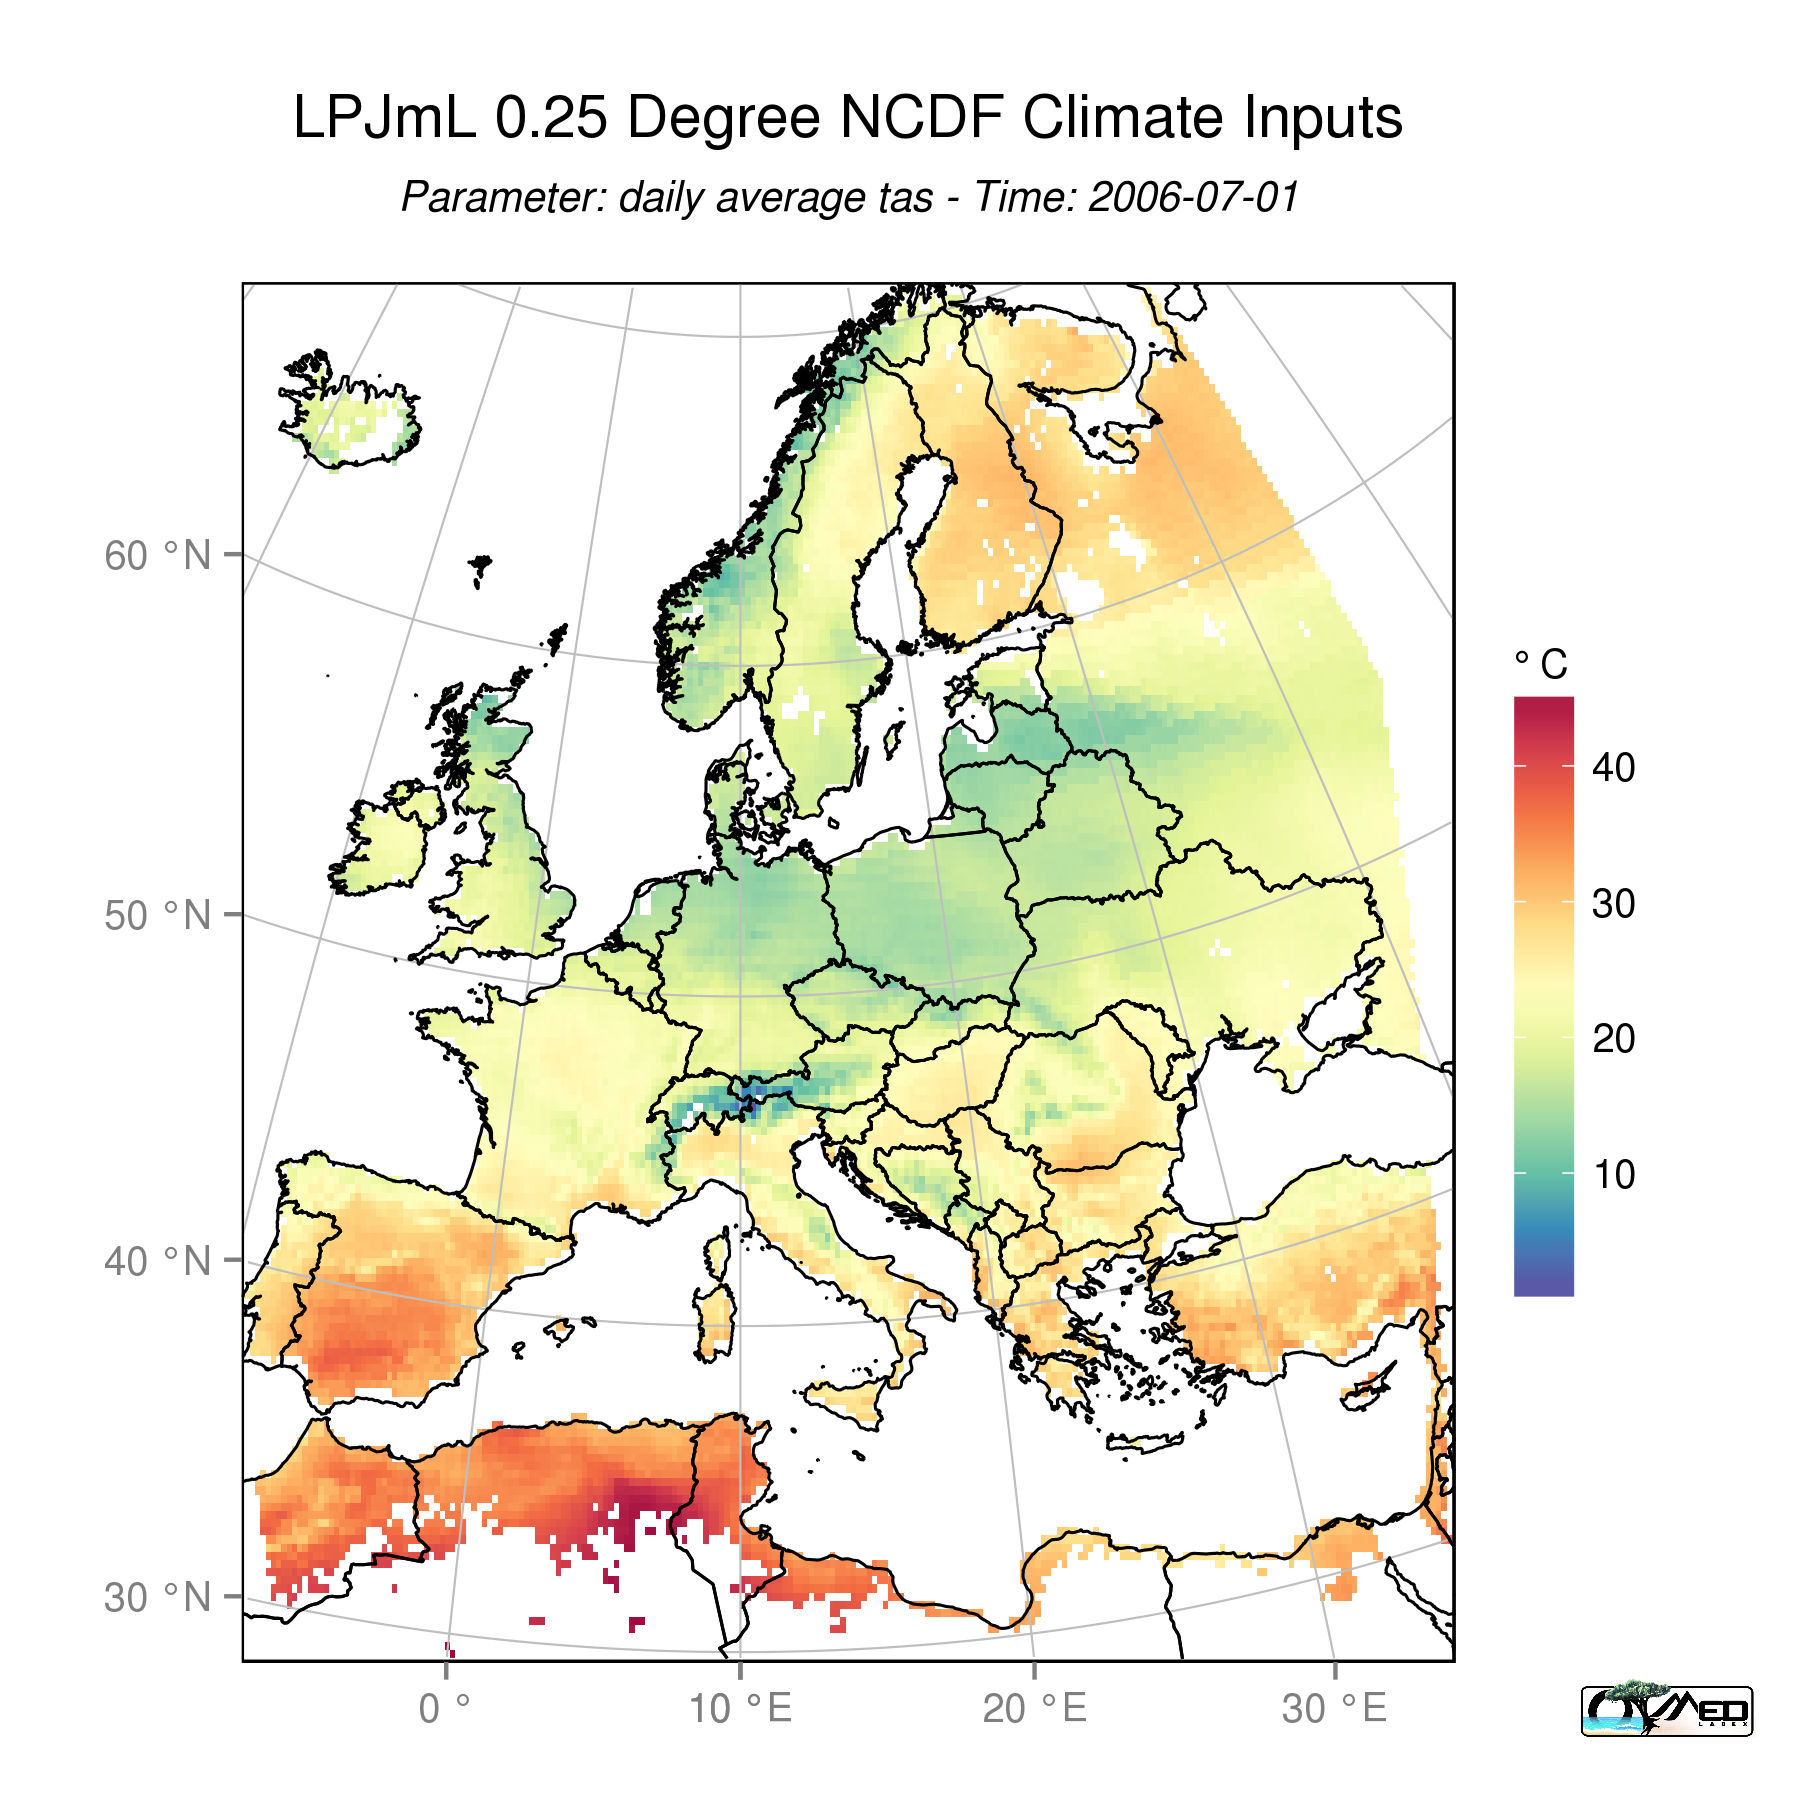
\includegraphics[width=1\textwidth]{first}
  \caption{Standard Map}
  \label{fig:gull}
\end{figure}
\subsection{Standard Map}
\subsection{Built in Polygons}
\subsection{Projections}
\subsection{Selecting Colour Scales}
\subsection{Colour Bars Position}
\subsection{Polygons Map}
\section{Further Development}
\subsection{Projection on irregular grids}












\end{document}



